\subsection{Orientation du courant}

\setcounter{equation}{0}
\setcounter{Q}{0}

On va s'intéresser à l'orientation du courant dans un accumulateur Li-ion constitué de deux électrodes où sont présents les couples suivants :

\begin{itemize}
\item  une électrode de graphite de couple redox \ce{C6}/\ce{LiC6} ;
\item une électrode d'oxyde de cobalt de couple redox \ce{CoO2}/\ce{LiCoO2}.
\end{itemize}

\Q Justifier l'appellation accumulateur.

\solution{
Si le système est un accumulateur, il est donc : 
\begin{itemize}
\item constitué d'un unique compartiment, par opposition au terme batterie ;
\item rechargeable, par opposition au terme pile.
\end{itemize}
}

\Q Montrer que chacun des couples est bien écrit sous la forme Ox/Réd en justifiant.

\solution{
On peut écrire pour chacun des couples :
\begin{align*}
\ce{C_6 + Li+ + e^- &= LiC6} \\
\ce{CoO2 + Li+ + e^- &= LiCoO2}
\end{align*}
En supposant un modèle purement ionique, on peut calculer la différence de degré d'oxydation entre l'état produit et l'état réactif :
\begin{align*}
\Delta no (\ce{C6}) &= -I < 0\\
\Delta no (\ce{Co}) &= - I < 0
\end{align*}
On a bien des réductions, donc les couples sont écrit sous la forme Ox/Réd.
}

\Q Donner l'équation de réaction fictive associée à ce système.

\solution{
On a au pôle $\ominus$ le graphite et au pôle $\oplus$ le cobalt. On en déduit donc que :
\begin{align*}
\ce{LiC6 + CoO2 = C6 + LiCoO2}
\end{align*}
On peut préciser que la notation ci-dessus sous-entend que tout le lithium migrera du graphite vers le cobalt.
On peut utiliser une notation intermédiaire en notant $x$ la stœchiométrie moyenne du lithium dans \ce{LiC6}, on peut aussi noter ce processus sous la forme : 
\begin{align*}
\ce{Li C6 + CoO2 = Li_x C6 + Li_{1-x}CoO2}
\end{align*}
Dans le cas présent, l'état produit est bien à un état intermédiaire entre l'état complètement chargé (resp. déchargé).
}

\Q En vous appuyant sur le schéma suivant, donner l'orientation de tous les flux dans la cellule en charge et en décharge.

\begin{center}
\begin{minipage}{0.48\textwidth}

\includegraphics[width=\textwidth]{Ex36/Fig01}
\end{minipage}\hfill\begin{minipage}{0.48\textwidth}
\captionof{figure}{Schéma d'un accumulateur li-ion}
\end{minipage}
\end{center}

\solution{On peut proposer l'orientation suivante :
\begin{center}
\begin{minipage}{0.48\textwidth}
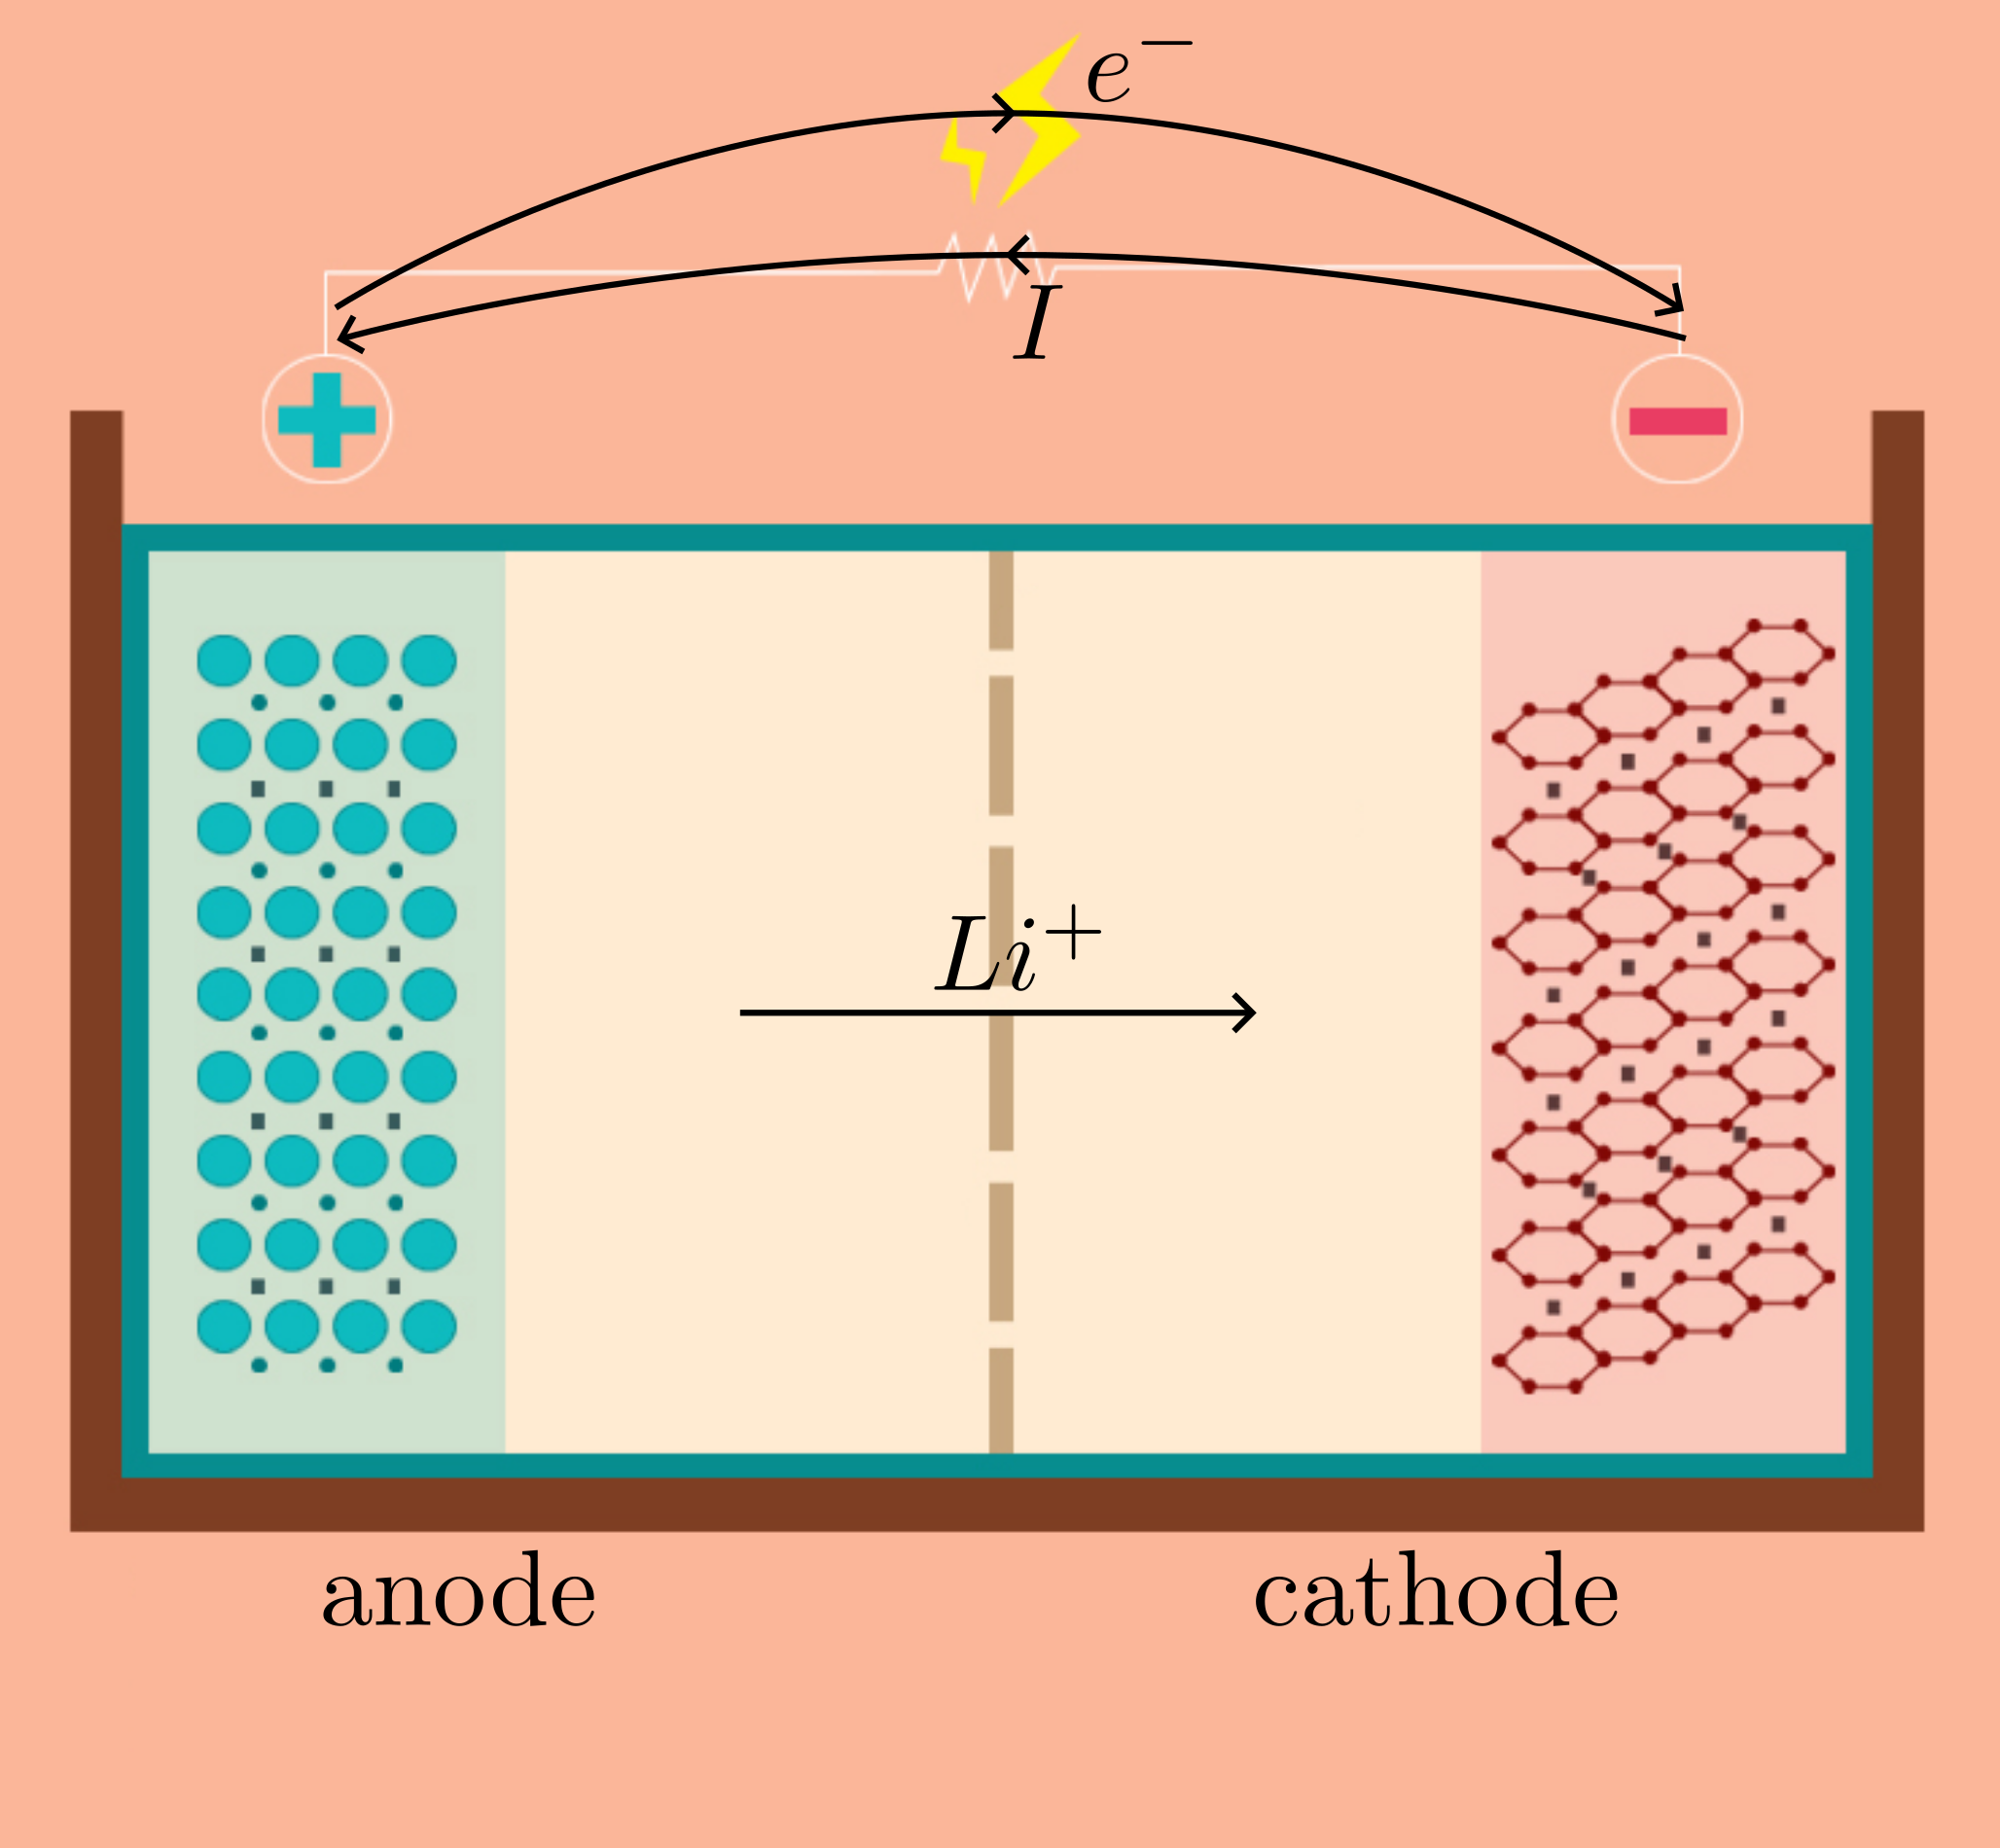
\includegraphics[width=\textwidth]{Ex36/Fig01-CorrectionCharge}\\
charge
\end{minipage}\hfill\begin{minipage}{0.48\textwidth}
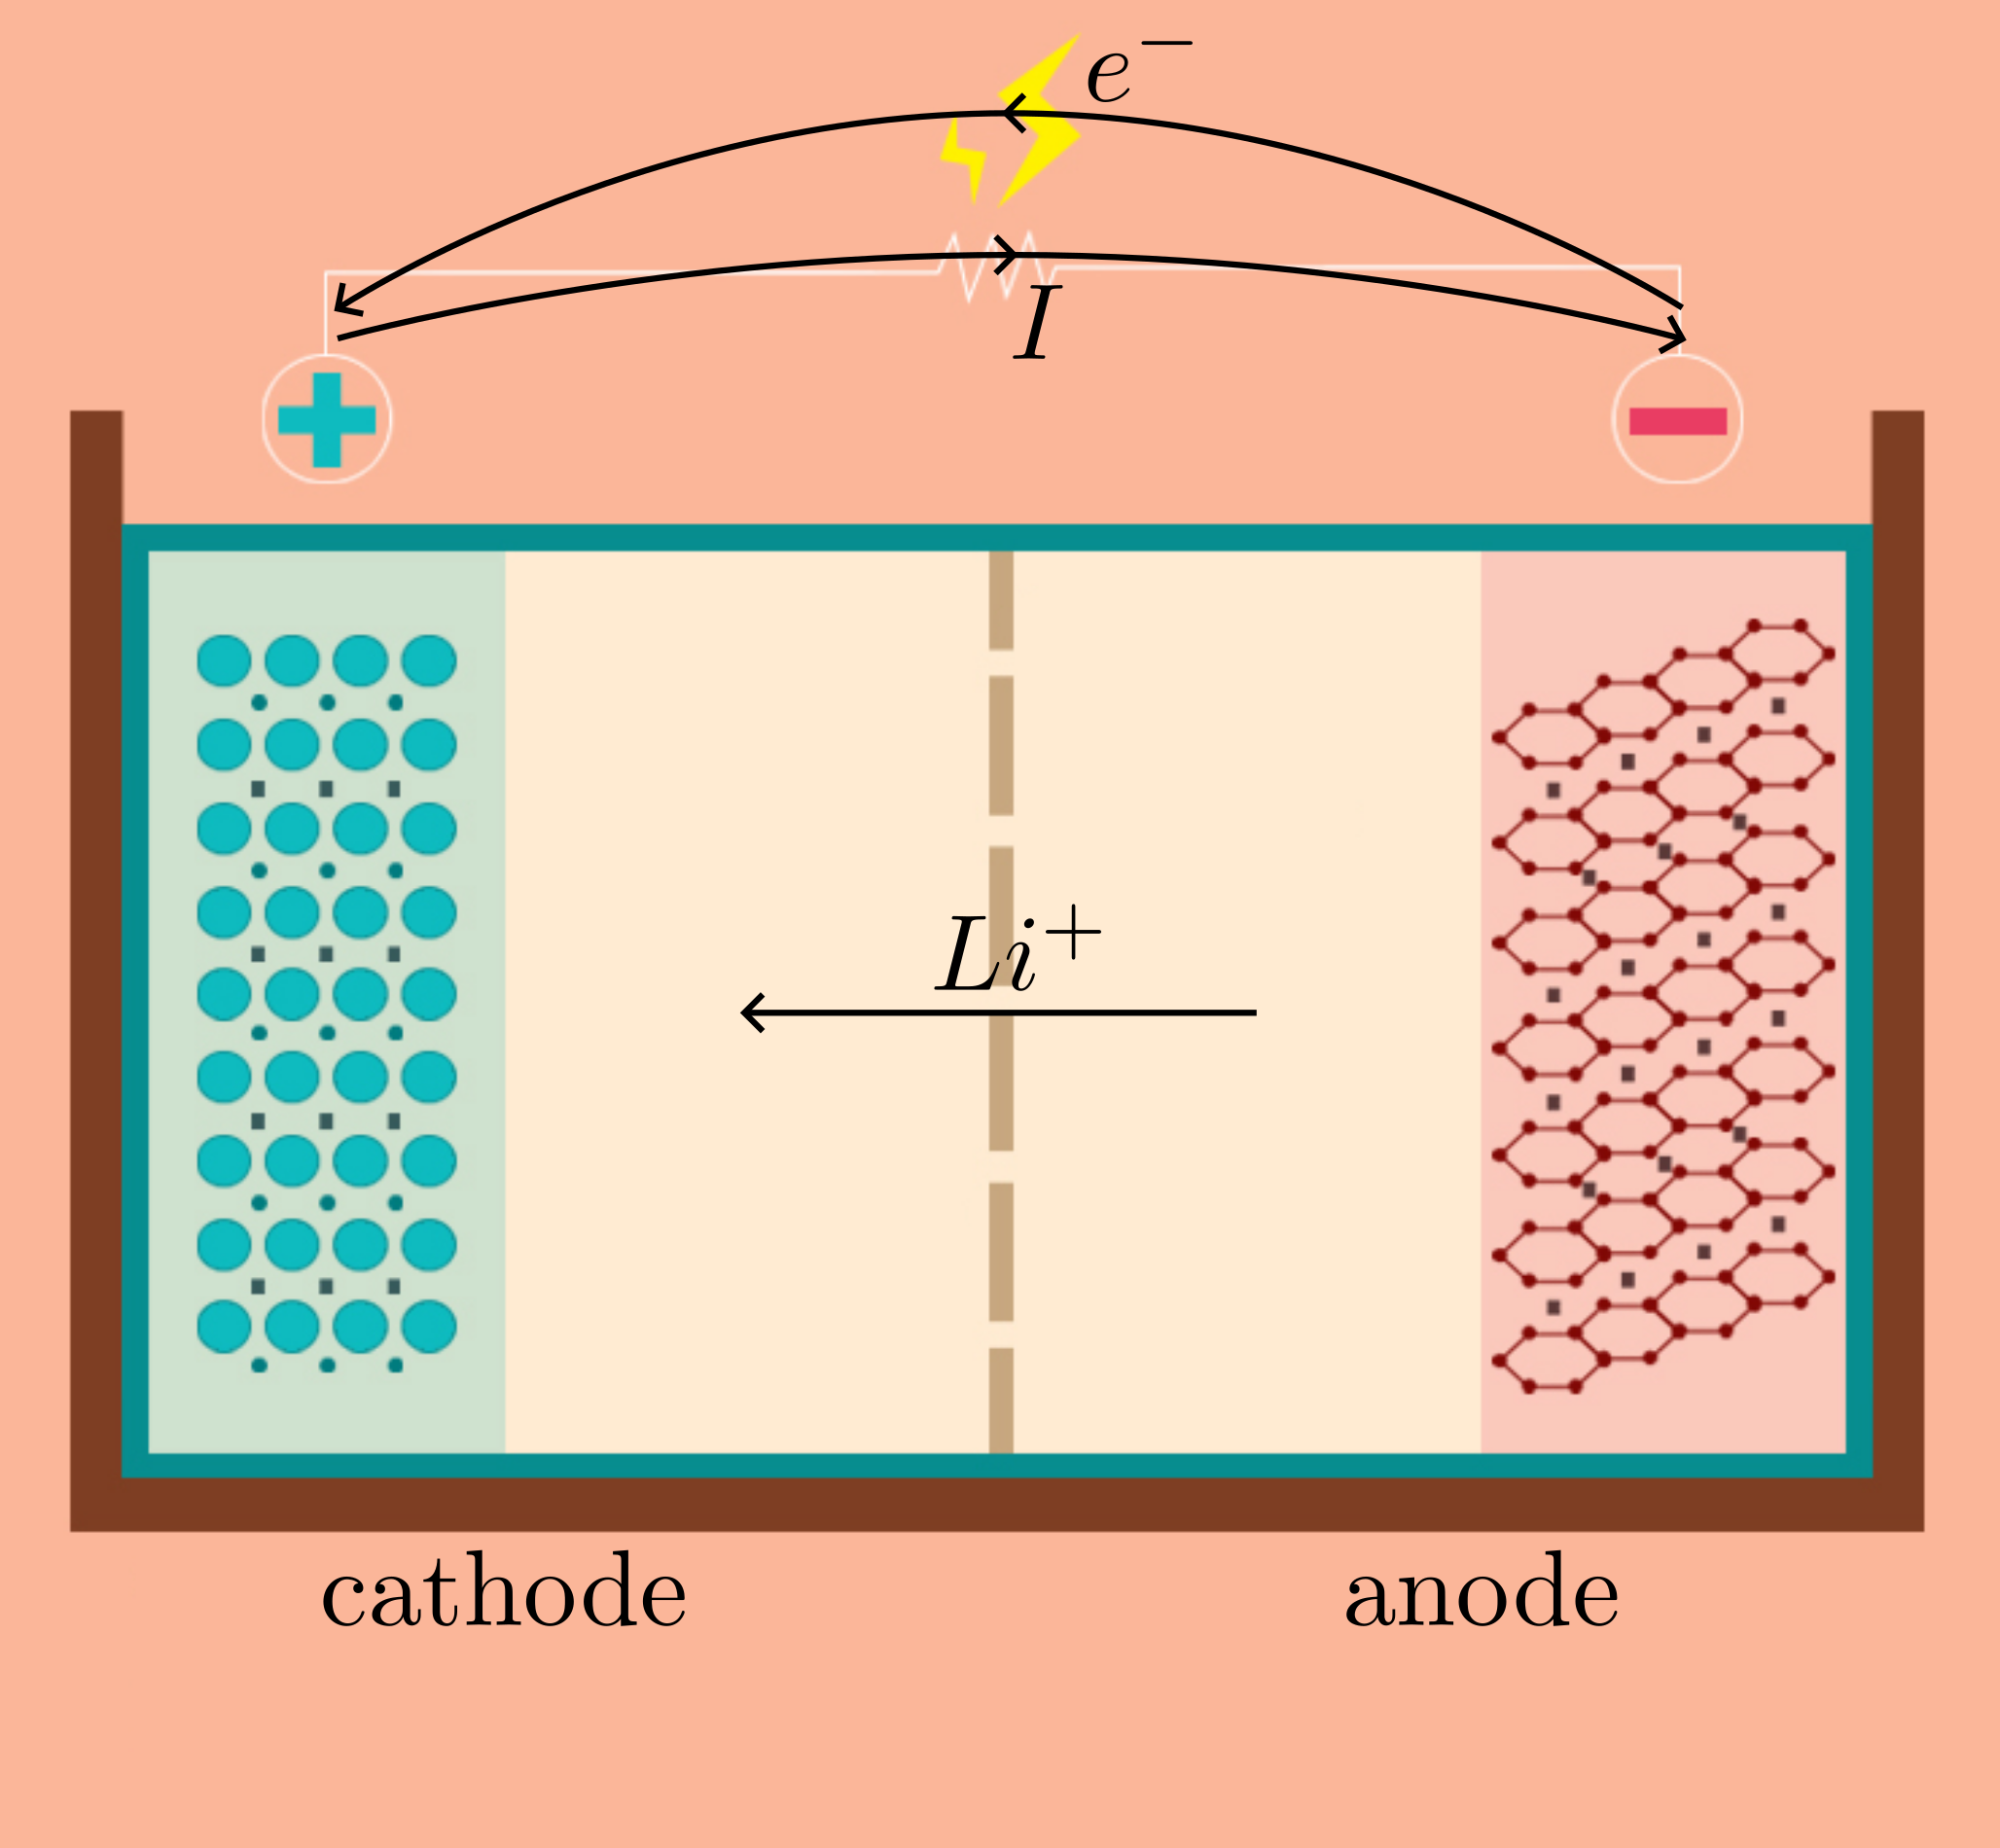
\includegraphics[width=\textwidth]{Ex36/Fig01-CorrectionDecharge} \\
décharge
\end{minipage}
\end{center}
Il faut se souvenir que le sens du courant imposé par la différence de potentiel, c'est-à-dire, la tension du générateur !
}